% Which rows enter the horizon-h regression in the twelve-period hand table.
% In each panel the lower line is the regression row t (it carries s_t and
% y_{t-1}); the upper line is the date whose outcome that row uses. The links
% shear right by h, so the last h rows point past t = 12 and leave the sample,
% and row 1 has no y_0. T_h = 12 - h - 1 = 11, 10, 9.
\documentclass[border=3pt]{standalone}
% ————— Shared preamble for the course figures —————
% Each figure is a standalone TikZ document. build.sh compiles it to a PDF (for
% the LaTeX build) and converts that to an SVG (for the web build).
%
% Nothing is drawn in pure black: the chrome sits at a mid grey that stays
% legible on white paper and on the site's dark theme alike. Data colours are
% the course palette, the same blue and orange used in the practicum.

\usepackage{amsmath}
\usepackage{tikz}
\usepackage{pgfplots}
\pgfplotsset{compat=1.18}
\usepgfplotslibrary{fillbetween,groupplots}
\usetikzlibrary{arrows.meta,positioning,calc,backgrounds}

\definecolor{nwBlue}{HTML}{2A78D6}
\definecolor{nwOrange}{HTML}{D9601F}
\definecolor{nwMut}{HTML}{898781}
\definecolor{nwInk}{HTML}{6B6965}

\pgfplotsset{
  nwaxis/.style={
    axis lines=left,
    axis line style={nwMut, line width=0.5pt},
    tick align=outside,
    tick style={nwMut, line width=0.5pt},
    label style={text=nwInk, font=\small},
    tick label style={text=nwMut, font=\footnotesize},
    legend cell align=left,
    legend style={draw=none, fill=none, font=\footnotesize, text=nwInk,
                  row sep=1pt, inner sep=1pt},
    every axis plot post/.append style={line join=round},
    clip mode=individual,
  },
}

\begin{document}
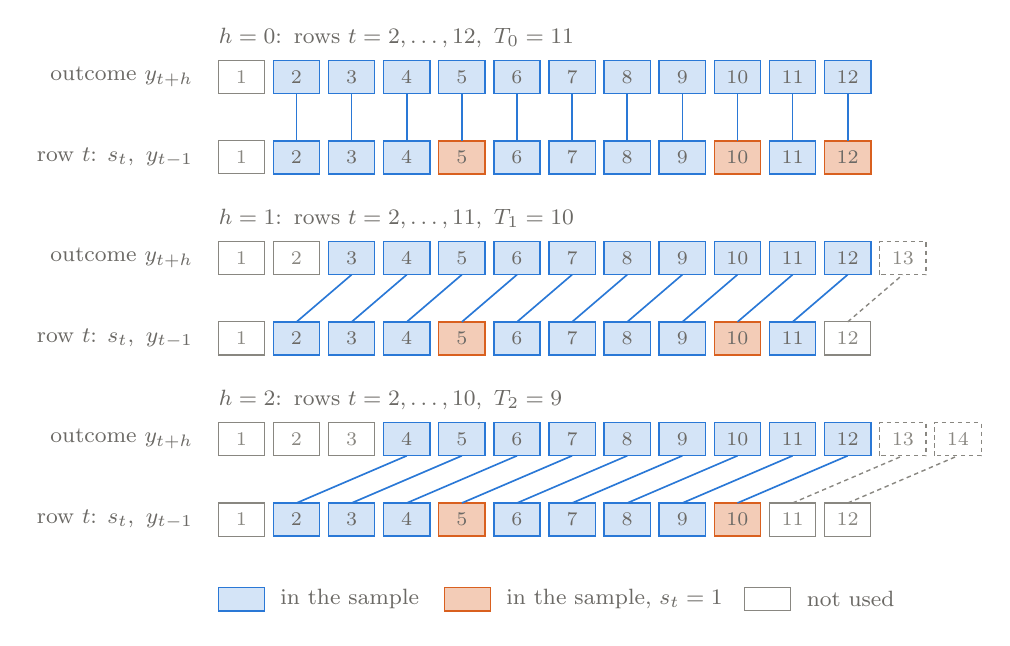
\begin{tikzpicture}[x=0.7cm, y=1cm,
  used/.style={fill=nwBlue!20, draw=nwBlue, line width=0.5pt},
  treat/.style={fill=nwOrange!32, draw=nwOrange, line width=0.5pt},
  idle/.style={fill=white, draw=nwMut, line width=0.4pt},
  ghost/.style={fill=none, draw=nwMut, line width=0.4pt, dash pattern=on 1.6pt off 1.3pt},
  num/.style={font=\scriptsize, inner sep=0pt},
  linelab/.style={text=nwInk, font=\footnotesize, anchor=east},
  head/.style={text=nwInk, font=\footnotesize, anchor=south west, inner sep=0pt},
  link/.style={draw=nwBlue, line width=0.6pt},
  lost/.style={draw=nwMut, line width=0.5pt, dash pattern=on 1.6pt off 1.3pt},
]

\def\G{0.08}    % half gap between cells, x units
\def\CH{0.42}   % cell height
\def\LG{0.6}    % link length
% shock dates of the hand table: s_t = 1 at t = 1, 5, 10, 12
\def\isshock#1{\ifnum#1=1 1\else\ifnum#1=5 1\else\ifnum#1=10 1\else\ifnum#1=12 1\else 0\fi\fi\fi\fi}

\foreach \hh/\base in {0/0, 1/-2.3, 2/-4.6} {
  \pgfmathtruncatemacro\last{12-\hh}
  \pgfmathtruncatemacro\first{2+\hh}
  \pgfmathtruncatemacro\Th{11-\hh}
  \pgfmathtruncatemacro\topd{12+\hh}
  \pgfmathsetmacro\yo{\base+\CH+\LG}          % bottom edge of the outcome line

  \node[head] at (0.5+\G,\yo+\CH+0.16)
    {$h=\hh$:\enspace rows $t=2,\dots,\last$,\enspace $T_{\hh}=\Th$};
  \node[linelab] at (0.3,\yo+0.5*\CH) {outcome $y_{t+h}$};
  \node[linelab] at (0.3,\base+0.5*\CH) {row $t$: $s_t,\ y_{t-1}$};

  % outcome line: dates 1..12 observed, beyond 12 not
  \foreach \dt in {1,...,\topd} {
    \ifnum\dt>12
      \draw[ghost] (\dt-0.5+\G,\yo) rectangle (\dt+0.5-\G,\yo+\CH);
      \node[num, text=nwMut] at (\dt,\yo+0.5*\CH) {\dt};
    \else\ifnum\dt<\first
      \draw[idle] (\dt-0.5+\G,\yo) rectangle (\dt+0.5-\G,\yo+\CH);
      \node[num, text=nwMut] at (\dt,\yo+0.5*\CH) {\dt};
    \else
      \draw[used] (\dt-0.5+\G,\yo) rectangle (\dt+0.5-\G,\yo+\CH);
      \node[num, text=nwInk] at (\dt,\yo+0.5*\CH) {\dt};
    \fi\fi
  }

  % regression rows
  \foreach \rw in {1,...,12} {
    \pgfmathtruncatemacro\tgt{\rw+\hh}
    \ifnum\rw<2
      \draw[idle] (\rw-0.5+\G,\base) rectangle (\rw+0.5-\G,\base+\CH);
      \node[num, text=nwMut] at (\rw,\base+0.5*\CH) {\rw};
    \else\ifnum\rw>\last
      \draw[idle] (\rw-0.5+\G,\base) rectangle (\rw+0.5-\G,\base+\CH);
      \node[num, text=nwMut] at (\rw,\base+0.5*\CH) {\rw};
      \draw[lost] (\rw,\base+\CH) -- (\tgt,\yo);
    \else
      \ifnum\isshock{\rw}=1
        \draw[treat] (\rw-0.5+\G,\base) rectangle (\rw+0.5-\G,\base+\CH);
      \else
        \draw[used] (\rw-0.5+\G,\base) rectangle (\rw+0.5-\G,\base+\CH);
      \fi
      \node[num, text=nwInk] at (\rw,\base+0.5*\CH) {\rw};
      \draw[link] (\rw,\base+\CH) -- (\tgt,\yo);
    \fi\fi
  }
}

% key
\begin{scope}[shift={(0.5+\G,-5.55)}]
  \draw[used]  (0,0) rectangle (0.84,0.3);
  \node[text=nwInk, font=\footnotesize, anchor=west] at (0.95,0.15) {in the sample};
  \draw[treat] (4.1,0) rectangle (4.94,0.3);
  \node[text=nwInk, font=\footnotesize, anchor=west] at (5.05,0.15) {in the sample, $s_t=1$};
  \draw[idle]  (9.55,0) rectangle (10.39,0.3);
  \node[text=nwInk, font=\footnotesize, anchor=west] at (10.5,0.15) {not used};
\end{scope}

\end{tikzpicture}
\end{document}
